\begin{problem}{별자리 3}
	{standard input}{standard output}
	{2 seconds}{512 megabytes}{}
	
	JOI군은 야경 사진을 찍었다. 이 사진은 가로 $N$개, 세로 $N$개의 픽셀로 되어있는 사진이다. 왼쪽에서 $x$ 번째 열, 아래에서 $y$ 번째 행 ($1 \le x \le N$, $1 \le y \le N$) 에 있는 픽셀을 픽셀 $(x, y)$ 라고 부른다.
	
	이 사진의 각 픽셀은 빌딩, 밤하늘 혹은 별이다. 색은 각각 하얀색, 검은색, 노란색이다. 각 $i$에 ($1 \le i \le N$) 대해 $i$번째 열에 있는 픽셀 중 아래에서 $A_i$행 까지는 하얀색 픽셀이다. 별이 찍힌 노란색 픽셀은 $M$개가 있고, 그 중 $j$ 번째 ($1 \le j \le M$) 픽셀은 픽셀 $(X_j, Y_j)$이다. 이 이외의 픽셀은 모두 밤하늘을 찍은 검은색 픽셀이다.
	
	이 사진의 어느 직사각형 영역이 다음 두 조건을 만족한다면 \textbf{별자리를 찍은 것}이 된다.
	
	\begin{itemize}
		\item 직사각형 영역 내에 하얀색 픽셀이 존재하지 않는다.
		\item 직사각형 영역 내에 노란색 픽셀이 두 개 이상 존재한다.
	\end{itemize}

	JOI군은 별자리를 보는 것이 지쳤다. 몇몇 노란색 픽셀을 검은색으로 칠하는 것으로 어떤 직사각형 영역도 별자리를 찍은 것이 되지 않도록 하고 싶다. 하지만 너무 많은 노란색 픽셀을 없애 버린 경우 사진의 \textbf{부자연스러움}이 올라간다. 구체적으로는 $j$ 번째 ($1 \le j \le M$) 노란색 픽셀을 검은색으로 만들면 사진의 부자연스러움이 $C_j$ 증가한다. 처음 사진의 부자연스러움은 0이다.
	
	사진의 정보와 각 노란색 픽셀을 없앴을 때 증가하는 부자연스러움이 주어졌을 때, 어떤 직사각형 영역도 별자리를 찍은 것이 되지 않도록 하면서 노란색 픽셀을 지운 사진의 부자연스러움의 최솟값을 구하는 프로그램을 작성하여라.
	
	
\InputFile

표준 입력에서 다음과 같은 형식으로 주어진다. 모든 값은 정수이다.

$N$ 

$A_1$ $\cdots$ $A_N$

$M$

$X_1$ $Y_1$ $C_1$

$\vdots$

$X_M$ $Y_M$ $C_M$

\OutputFile

어떤 직사각형 영역도 별자리를 찍은 것이 되지 않도록 하면서 노란색 픽셀을 지울 때, 사진의 부자연스러움의 최솟값을 표준 출력으로 첫째 줄에 출력하여라.

\Constraints

\begin{itemize}
	\item $1 \le N \le 200\ 000$.
	\item $1 \le A_i \le N$ ($1 \le i \le N$).
	\item $1 \le M \le 200\ 000$.
	\item $1 \le X_j \le N$ ($1 \le j \le M$).
	\item $1 \le Y_j \le N$ ($1 \le j \le M$).
	\item $1 \le C_j \le 1\ 000\ 000\ 000$ ($1 \le j \le M$).
	\item $A_{X_j} < Y_j$ ($1 \le j \le M$).	
	\item $(X_j, Y_j) \ne (X_k, Y_k)$ ($1 \le j < k \le M$).
\end{itemize}


\SubtaskWithCost{1}{14}
\begin{itemize}
	\item $N \le 300$.
	\item $M \le 300$.
\end{itemize}


\SubtaskWithCost{2}{21}
\begin{itemize}
	\item $N \le 2\ 000$.
	\item $M \le 2\ 000$.
\end{itemize}

\SubtaskWithCost{3}{65}

추가 제한조건이 없다.

\Examples

\begin{example}
	\exmp{
		5
		1 3 4 2 3
		3
		1 5 3
		4 3 2
		2 4 2
	}{%
		2
	}%
\end{example}

이 입력 예제에서, 픽셀 $(1, 5)$을 왼쪽 아래의 정점, 픽셀 $(2, 4)$를 오른쪽 아래의 정점으로 하는 직사각형 영역은 별자리를 찍은 것이다. 세 번째 노란색 픽셀을 검은색으로 만들면 사진의 부자연스러움은 2 증가하고 어떤 직사각형 영역도 별자리를 찍은 것이 되지 않는다. 이것이 최솟값이므로 2를 출력한다.

이 입력 예제의 사진은 (그림 1)에 대응된다.

\begin{center}
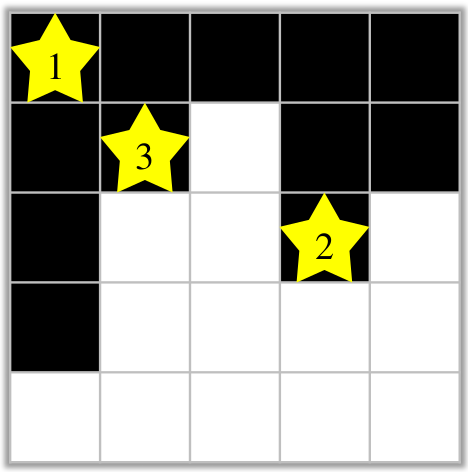
\includegraphics[width=0.3\linewidth]{img1.png}

그림 1
\end{center}


\begin{example}
	\exmp{
		7
		5 6 2 3 6 7 6
		5
		7 7 5
		3 3 7
		3 7 10
		1 7 6
		4 7 8
	}{%
		16
	}%
\end{example}

이 입력 예제에서, 세 번째와 네 번째 노란색 픽셀을 검은색으로 만들면 된다.

\begin{example}
	\exmp{
		8
		6 8 5 7 3 4 2 1
		10
		8 2 9
		6 6 7
		8 3 18
		5 8 17
		8 5 3
		5 5 3
		5 4 8
		1 8 13
		1 7 5
		7 4 13
	}{%
		44
	}%
\end{example}


\end{problem}

